\chapter{Stage 3 Integrated: Combined Grid and Sensitivity}
\label{ch:stage3_integrated}

Stage 3 Integrated merges the brightness-constrained view (Chapter~\ref{ch:stage3a})
and the optical-quality view (Chapter~\ref{ch:mtf_strehl}) onto one shared
$(a_{hole}, M)$ grid --- a pandas join on real, independently-computed physics outputs
from both, not a new model of its own.

\begin{figure}[htbp]
\centering
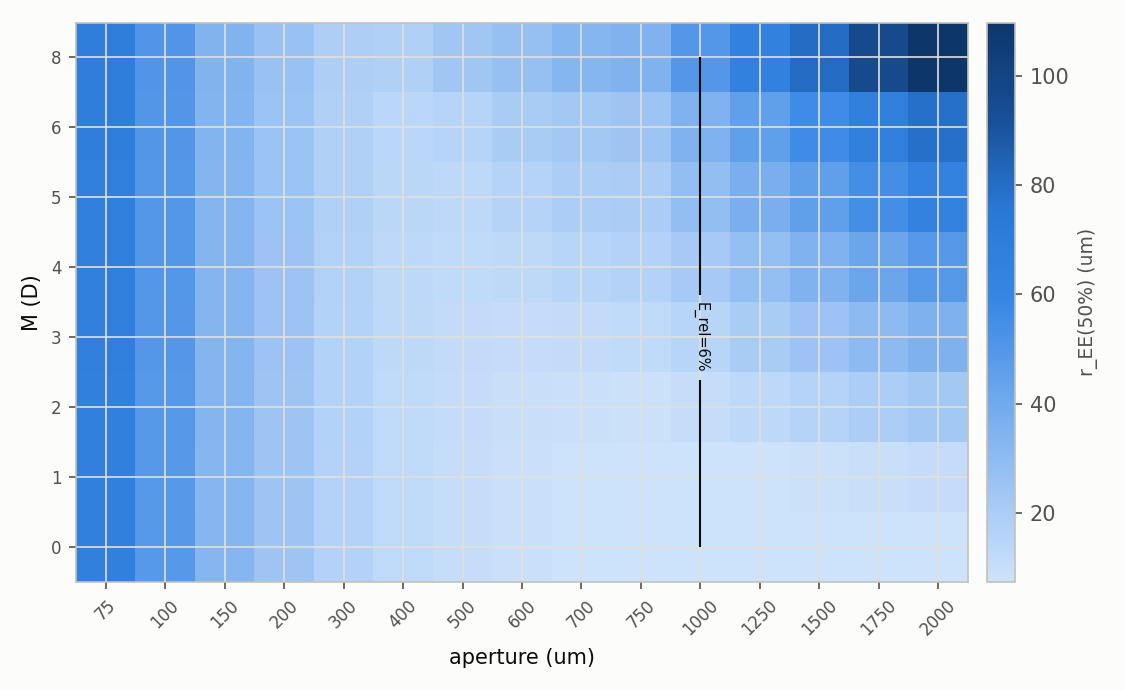
\includegraphics[width=0.85\textwidth]{figures/fig_stage3_integrated_heatmap.png}
\caption{Combined view: $r_{EE}(50\%)$ (color) with relative illuminance $E_{rel}$ contours overlaid, across the full grid.}
\label{fig:stage3-integrated}
\end{figure}

This combined view makes visible, on one figure, exactly the trade-off
Chapters~\ref{ch:r1sweep} and~\ref{ch:stage3a} describe separately: the blur-optimal
region (small apertures) and the brightness-adequate region (large apertures) occupy
opposite corners of the grid at low myopia, and the two regions move closer together
as myopia increases (since the blur-optimal aperture itself grows with the geometric
defocus at low-to-moderate $M$, per Chapter~\ref{ch:r1sweep}'s own U-shaped curves).
\textbf{Correctness caveat, stated explicitly}: this merge is valid only when both legs
share the same wavelength/gap/pupil parameters, which this report's sweeps do
throughout; the underlying tool does not itself prevent mismatched parameters if a
reader were to select them independently.
